\section{Mathematical Models}
\label{ch:mathmodel}

As per the base and periodic models shown in \cite{grigor20}.

\subsection{Base model}

The majority of the definitions and results are in \label{ch:theorems}.

\subsubsection{How to select the best model}

\begin{figure}[H]
\minipage{0.33\textwidth}
  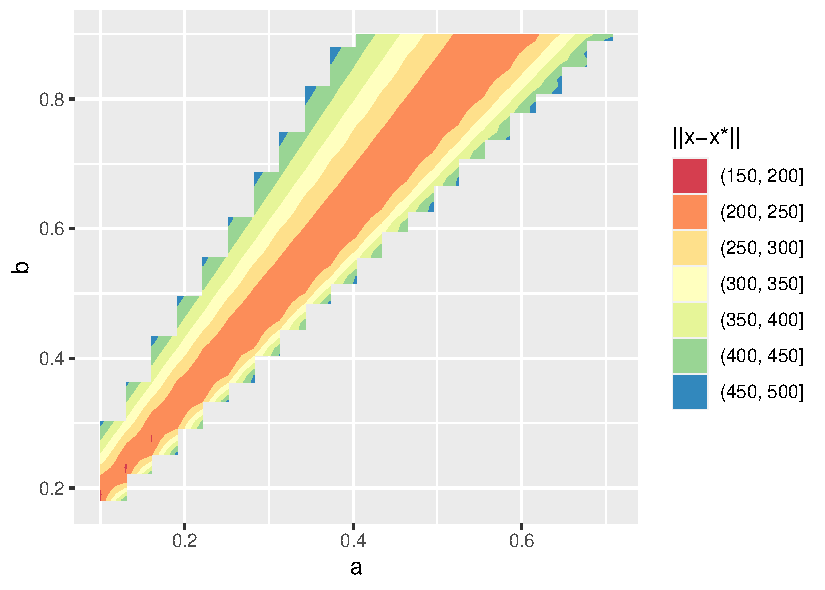
\includegraphics[width=\linewidth]{Ireland-combnorm.pdf} \label{fig:ireland-combnorm}
\caption{Contours, Ireland}
\endminipage\hfill
\minipage{0.33\textwidth}
  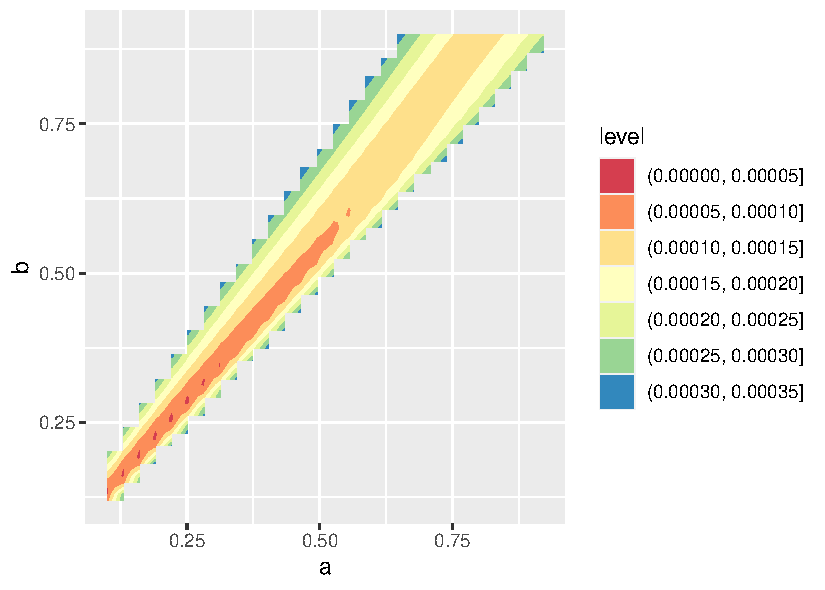
\includegraphics[width=\linewidth]{Italy-combnorm.pdf} \label{fig:italy-combnorm}
\caption{Contours, Italy}
\endminipage\hfill
\minipage{0.33\textwidth}
  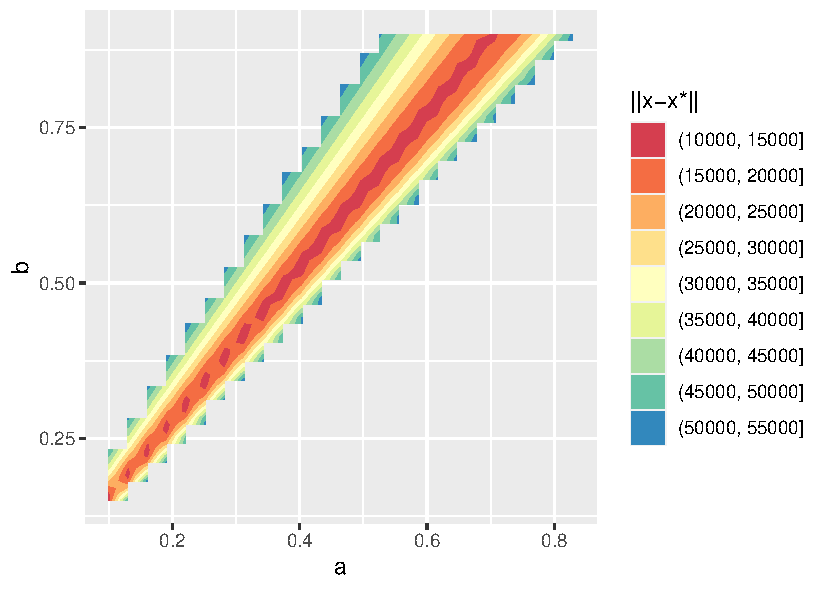
\includegraphics[width=\linewidth]{United States-combnorm.pdf} \label{fig:usa-combnorm}
\caption{Contours, United States}
\endminipage\hfill
\end{figure}

\subsubsection{Forecasting}

\subsubsection{Implementation in R}

\begin{lstlisting}[breaklines = true, escapeinside=||, tabsize = 4, caption = {Algorithm for Base Model}]
basicmodx <- function(x, pars, len = 0){
  q <- floor(pars[1])
  a <- pars[2]
  b <- pars[3]
  modx <- x[1:q]
  for(i in (q+1):(length(x)+len)){
    modx[i] <- (1-b)*modx[i-1] + a*modx[i-q]
  }
  return(modx)
}
basexn   <- basicmodx(countrydat$xn, optimpars, len = forecastlen)  |\Suppressnumber|
...
...
...|\Reactivatenumber|
plots[["basexn"]] <- plot_basexn(countrydat, modeldat, cols, labs)
\end{lstlisting}

\subsubsection{Plots}

\begin{figure}[H]
\minipage{0.48\textwidth}
  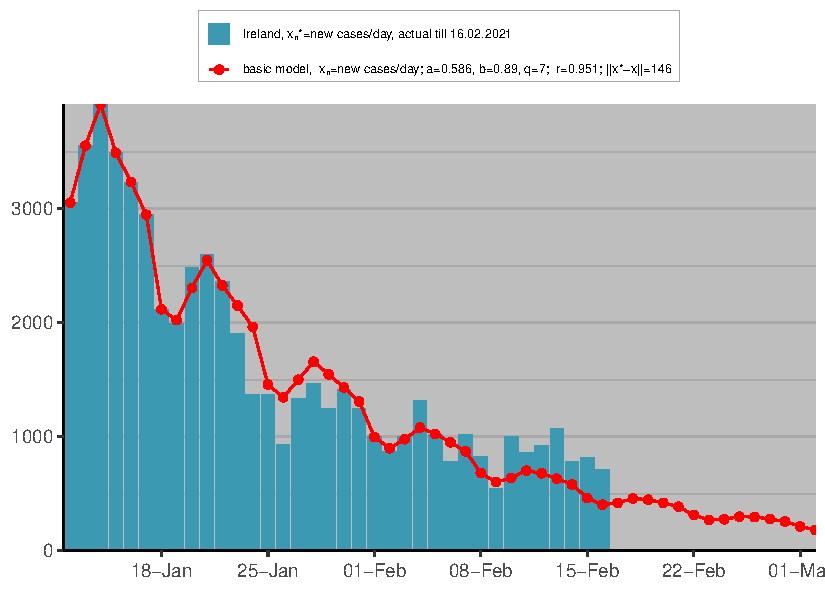
\includegraphics[width=\linewidth]{Ireland-basexn.pdf} \label{fig:ireland-basexn}
\endminipage\hfill
\minipage{0.48\textwidth}
  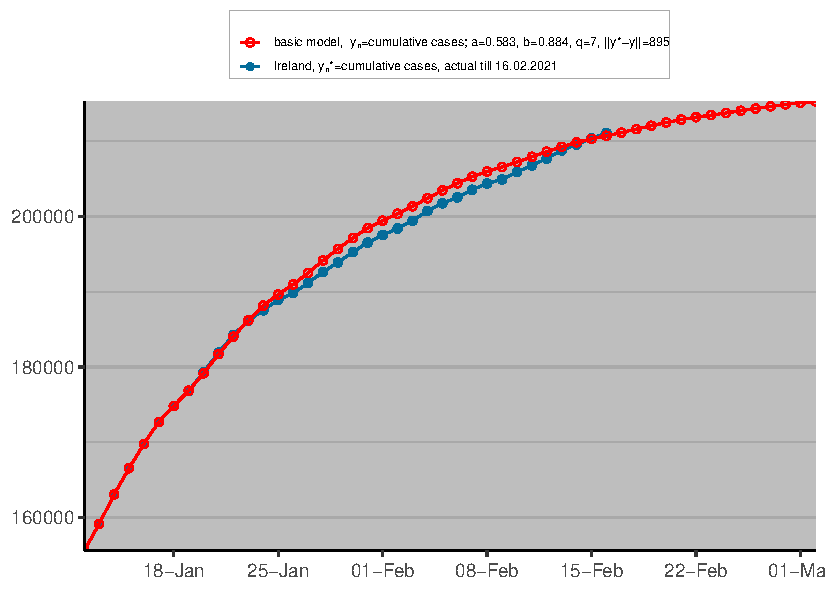
\includegraphics[width=\linewidth]{Ireland-baseyn.pdf} \label{fig:ireland-baseyn}
\endminipage
\caption{Basic model, Ireland}
\end{figure}

\begin{figure}[H]
\minipage{0.48\textwidth}
  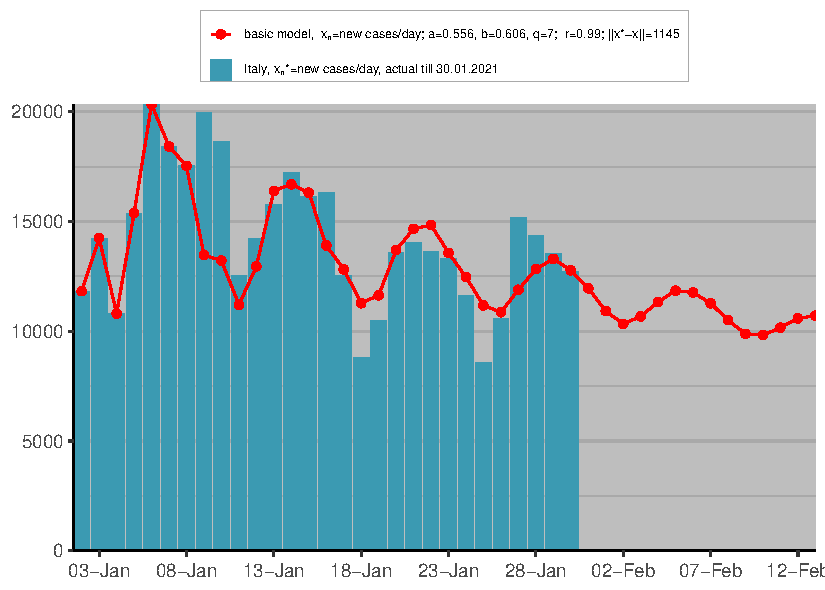
\includegraphics[width=\linewidth]{Italy-basexn.pdf} \label{fig:italy-basexn}
\endminipage\hfill
\minipage{0.48\textwidth}
  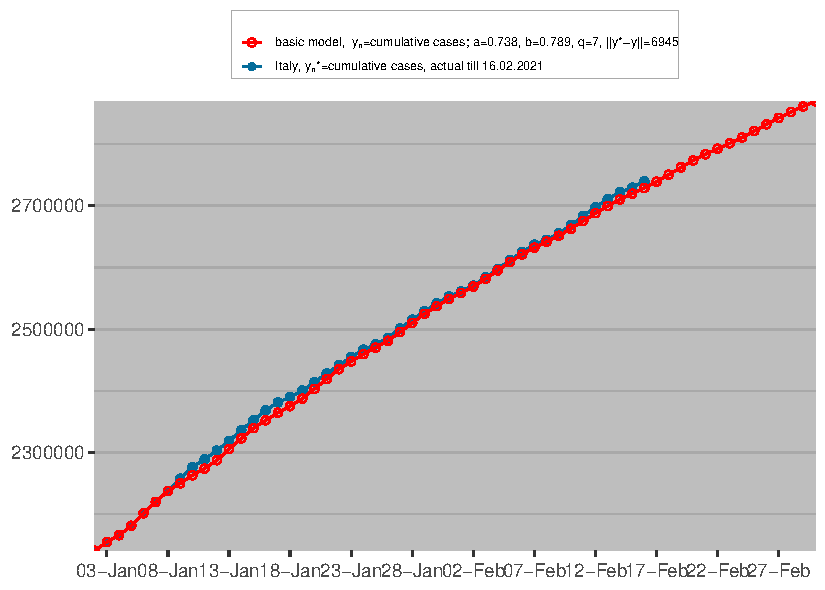
\includegraphics[width=\linewidth]{Italy-baseyn.pdf} \label{fig:italy-baseyn}
\endminipage
\caption{Basic model, Italy}
\end{figure}

\begin{figure}[H]
\minipage{0.48\textwidth}
  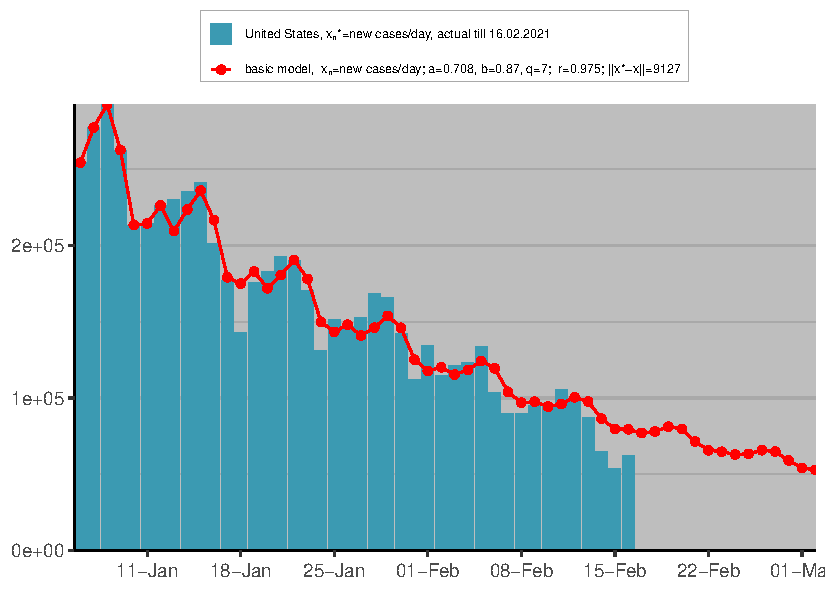
\includegraphics[width=\linewidth]{United States-basexn.pdf} \label{fig:usa-basexn}
\endminipage\hfill
\minipage{0.48\textwidth}
  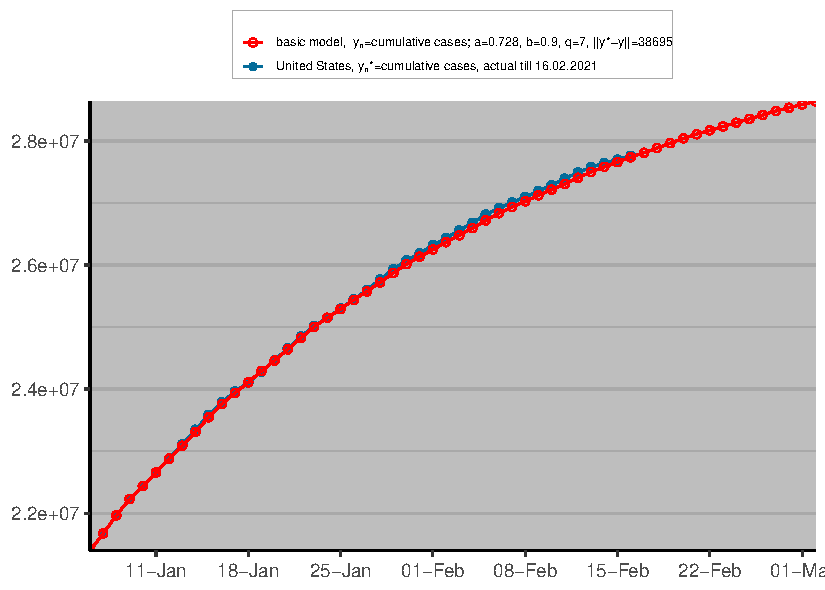
\includegraphics[width=\linewidth]{United States-baseyn.pdf} \label{fig:usa-baseyn}
\endminipage
\caption{Basic model, United States}
\end{figure}

\subsection{Limiting curve}

The second result in \ref{thm:lim} is the equation \ref{eq:crn}, which defines the limiting behavior of the recurrence relation \ref{eq:an}.

\begin{lstlisting}[breaklines = true, escapeinside=||, tabsize = 4, caption = {Algorithm for Limiting Curve}]
modeldat$Crn <- optimC*base_r_one^(1:nrow(modeldat))  |\Suppressnumber|
...
...
...|\Reactivatenumber|
plots[["Crn"]] <- plot_crn(countrydat, modeldat, cols, labs)
\end{lstlisting}

\begin{figure}[H]
\minipage{0.33\textwidth}
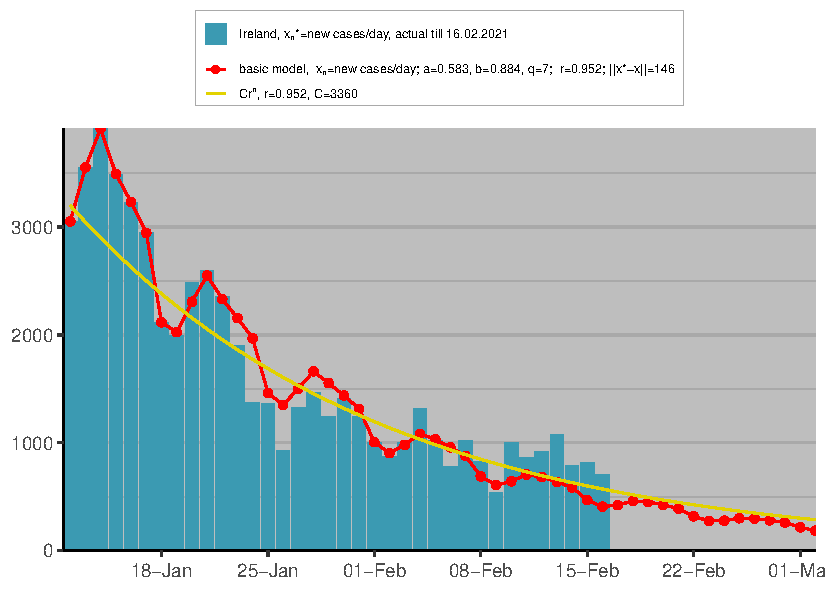
\includegraphics[width=0.9\textwidth]{Ireland-Crn.pdf}
\caption{Limiting curve $Cr^n$, Ireland}
\endminipage 
\minipage{0.33\textwidth}
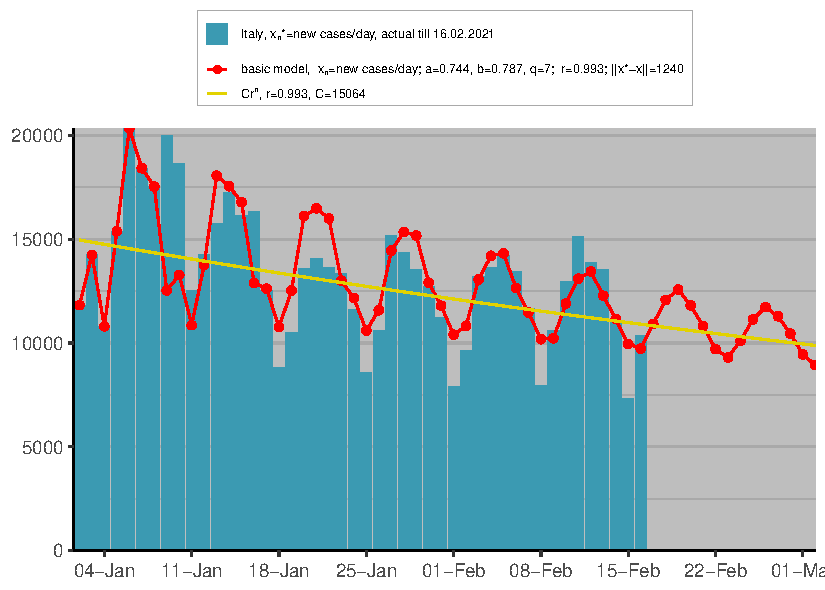
\includegraphics[width=0.9\textwidth]{Italy-Crn.pdf}
\caption{Limiting curve $Cr^n$, Italy}
\endminipage 
\minipage{0.33\textwidth}
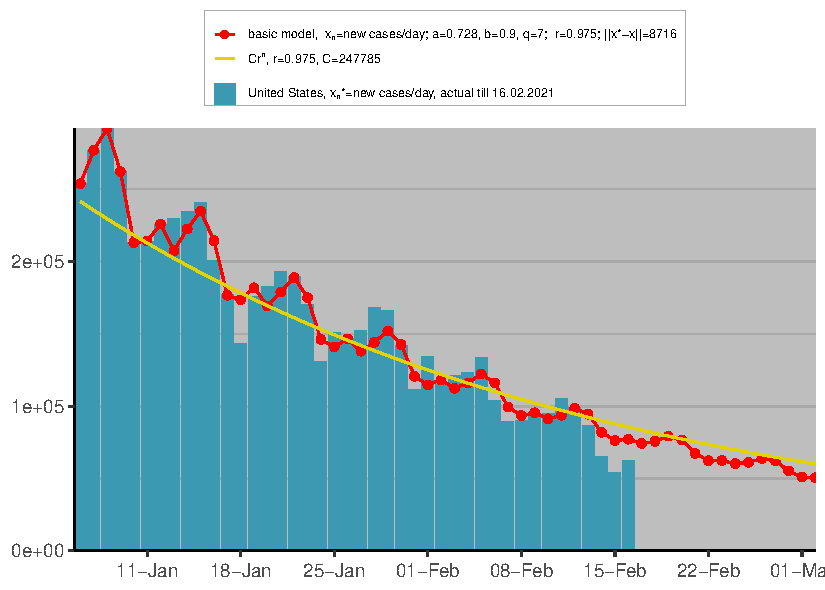
\includegraphics[width=0.9\textwidth]{United States-Crn.pdf}
\caption{Limiting curve $Cr^n$, United States}
\endminipage 
\end{figure}

The limiting curve can of course so exponential growth 

\begin{figure}[H]
\minipage{0.98\textwidth}
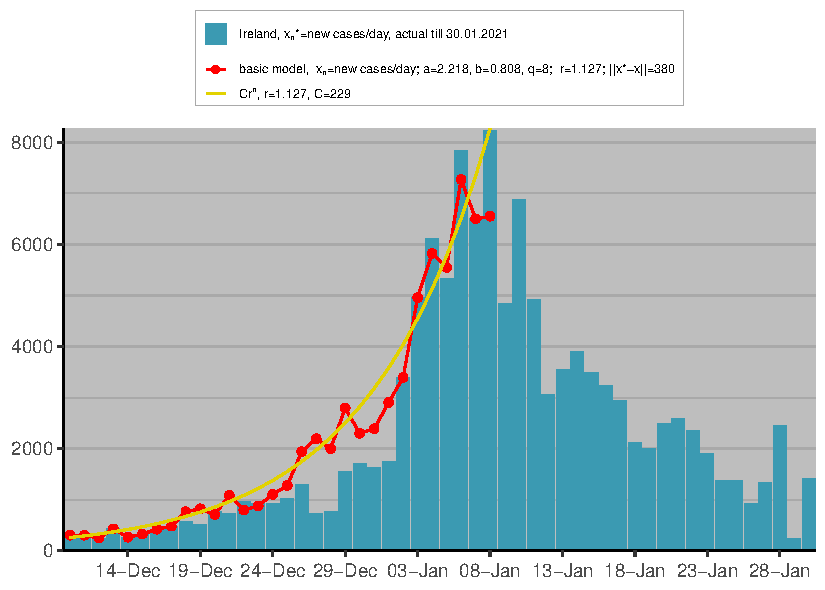
\includegraphics[width=0.9\textwidth]{Ireland-expgrowth.pdf}
\endminipage 
\caption{Limiting Curve Growing Exponentially, Ireland}
\end{figure}

\subsection{Moving average}

Define the $2k+1$-day moving average of actual data $x_n^*$ by $x^*(k)$

$\begin{aligned}
x^*_n(1) &=\frac{x^*_{n-1} + x^*_n + x^*_{n+1}}{3},\quad 1\leq n < N \\
x^*_0(1) &=\frac{x^*_0 + x^*_1}{2}\\
x^*_N(1) &=\frac{x^*_{N-1} + x^*_N}{2}
\end{aligned}$

And then $$x_n^*(3):= x^*_n(x^*_n(1))$$ is the 7-day moving average of cases.

The 7-day moving average is a good baseline for model performance , as ideally we would want $\norm{x-x^*}\approx\norm{x^*(3)-x^*}$ or better.

\begin{figure}[H]
\minipage{0.33\textwidth}
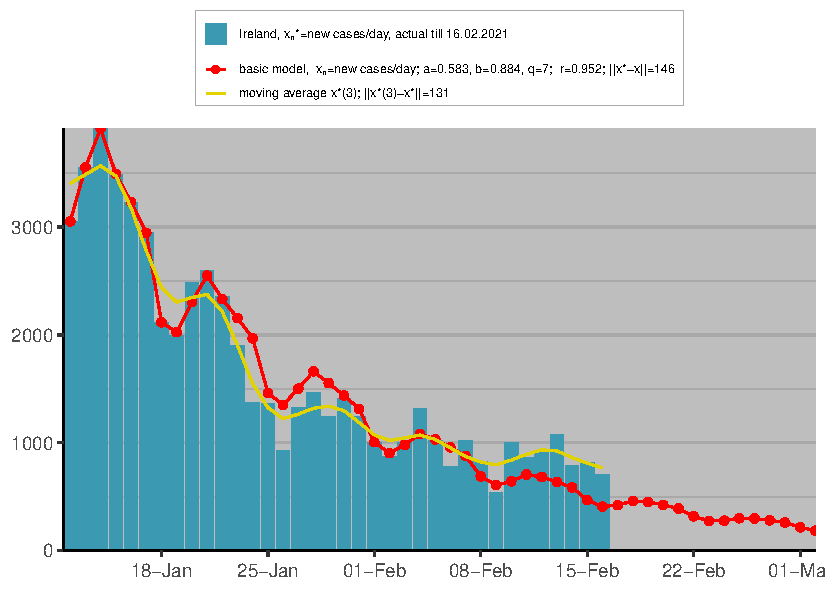
\includegraphics[width=0.9\textwidth]{Ireland-mavgx3.pdf}
\caption{Moving average $x^*_n (3)$, Ireland}
\endminipage 
\minipage{0.33\textwidth}
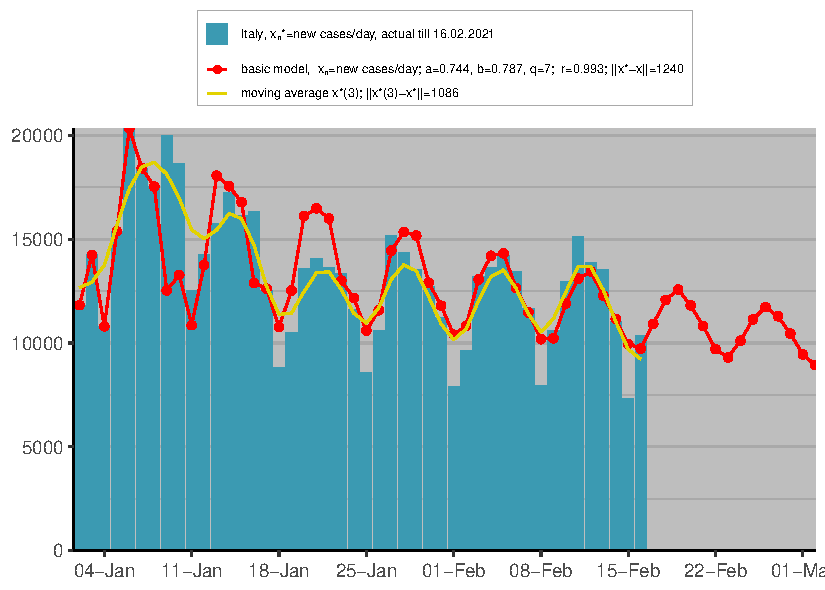
\includegraphics[width=0.9\textwidth]{Italy-mavgx3.pdf}
\caption{Moving average $x^*_n (3)$, Italy}
\endminipage 
\minipage{0.33\textwidth}
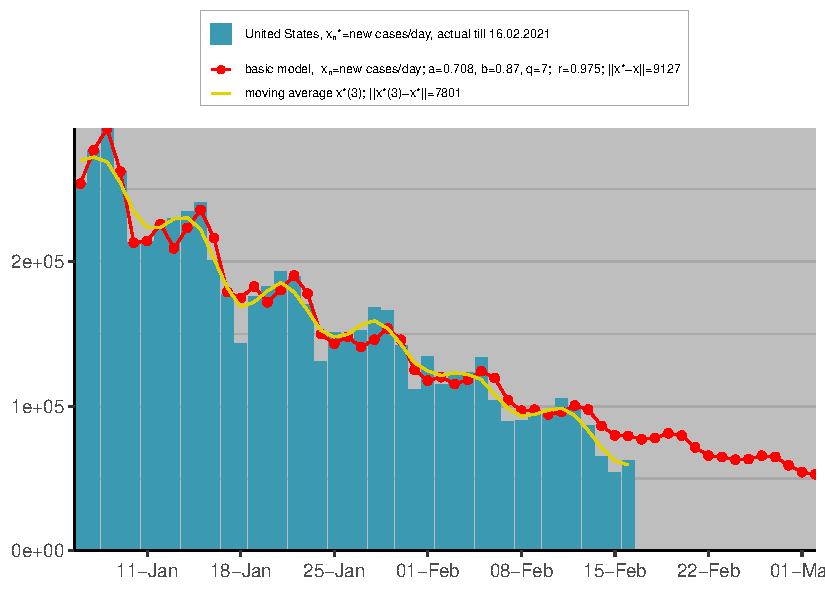
\includegraphics[width=0.9\textwidth]{United States-mavgx3.pdf}
\caption{Moving average $x^*_n (3)$, United States}
\endminipage 
\end{figure}

\subsection{Periodic model}

\subsubsection{Definitions and Theory}

Instead of constant parameters $a,b$, we vary them slightly over time:

$a_n := a\rbr{1+c_1\rbr{\sin\rbr{\frac{2\pi}{p_1}\rbr{n-n_1}}}}$

$b_n := b\rbr{1+c_2\rbr{\sin\rbr{\frac{2\pi}{p_2}\rbr{n-n_2}}}}$

For new parameters $c_i,p_i,n_i, \ i=1,2$ where

$c_i  \in [0.04, 0.2] \quad \text{small}$

$n_i  \in 1,2,\dots,q$

$p_i  \in 1,2,\dots,q$

\begin{figure}[H]
\minipage{0.33\textwidth}
  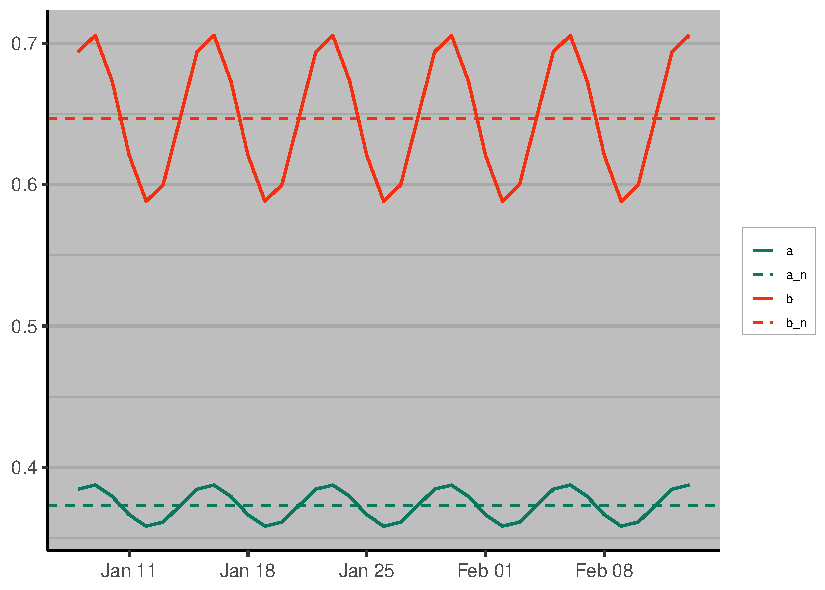
\includegraphics[width=\linewidth]{Ireland-perparam.pdf} \label{fig:ireland-perparam}
\endminipage\hfill
\minipage{0.33\textwidth}
  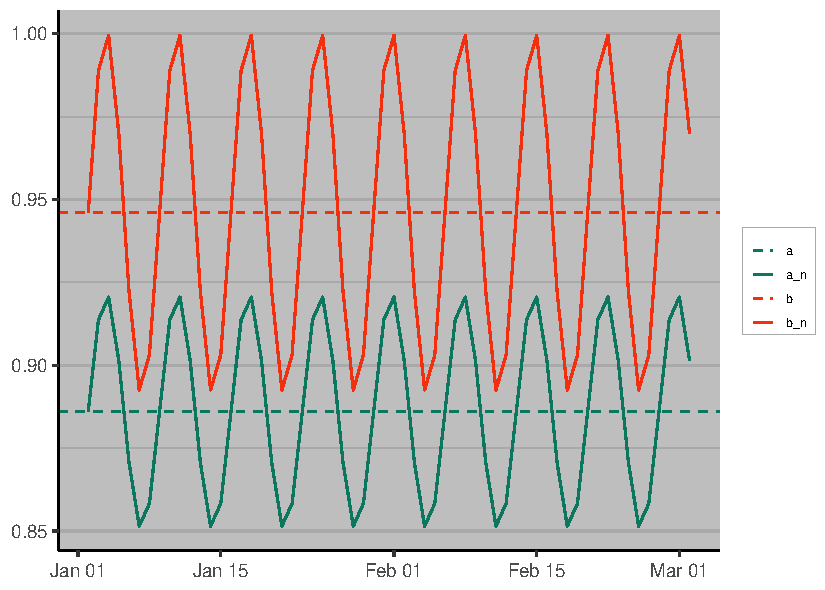
\includegraphics[width=\linewidth]{Italy-perparam.pdf} \label{fig:italy-perparam}
\endminipage\hfill
\minipage{0.33\textwidth}
  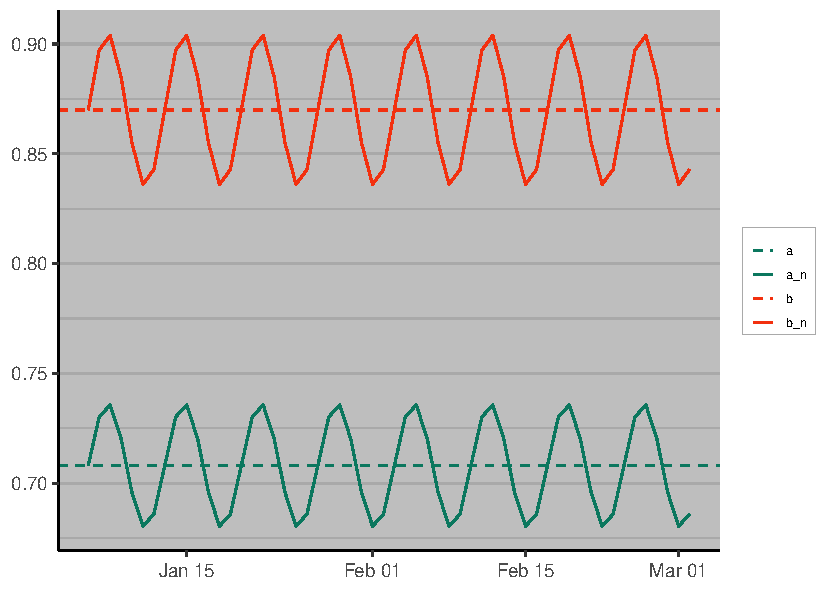
\includegraphics[width=\linewidth]{United States-perparam.pdf} \label{fig:usa-perparam}
\endminipage\hfill
\caption{Oscillating $a$ and $b$ parameters, Ireland, Italy and United States}
\end{figure}

\subsubsection{Implementation in R}

\begin{lstlisting}[breaklines = true, escapeinside=||, tabsize = 4, frame=single, caption = {Algorithm for Periodic Model}]
modxper <- function(par, q, x, len = 0){
  #a,b,c1,c2,p1,p2,n1,n2
  an   <- par[1]*(1+par[3]*sin(2*pi*(1:(length(x)+len) - par[7])/par[5]))
  bn   <- par[2]*(1+par[4]*sin(2*pi*(1:(length(x)+len) - par[8])/par[6]))
  modx <- x[1:q]
  for(i in (q+1):(length(x)+len)){
    modx[i] <- (bn[i]*(1-bn[i-1]))*modx[i-1]/bn[i-1] +
      (an[i-q]*bn[i])*modx[i-q]/bn[i-q]
  }
  return(modx)
}
modeldat$periodic  <- modxper(as.numeric(peroptim),countrydat$xn, q = q, forecastlen)|\Suppressnumber|
...
...
...|\Reactivatenumber|
plots[["periodic"]] <- plot_periodic(countrydat, modeldat, cols, labs)
\end{lstlisting}

\subsubsection{Plots}

\begin{figure}[H]
\minipage{0.48\textwidth}
  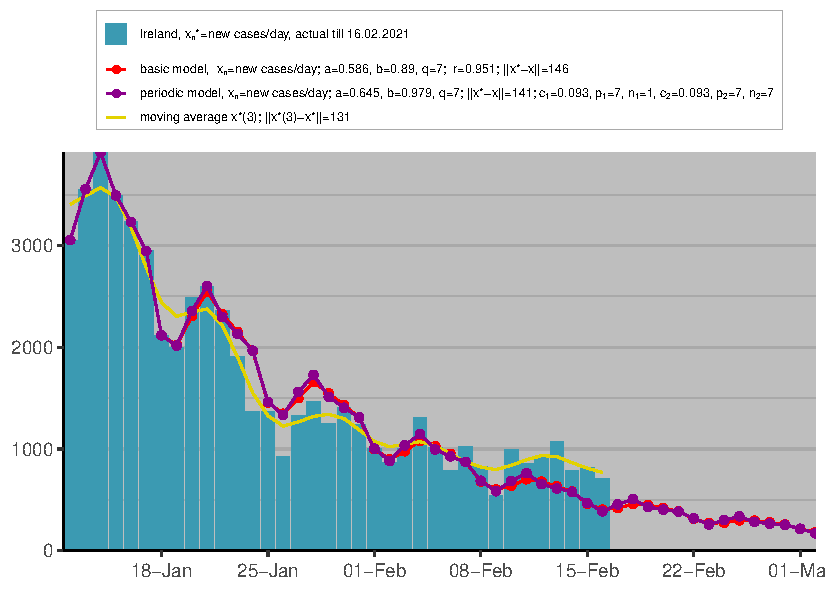
\includegraphics[width=\linewidth]{Ireland-periodic.pdf} \label{fig:ireland-periodic}
\endminipage\hfill
\minipage{0.48\textwidth}
  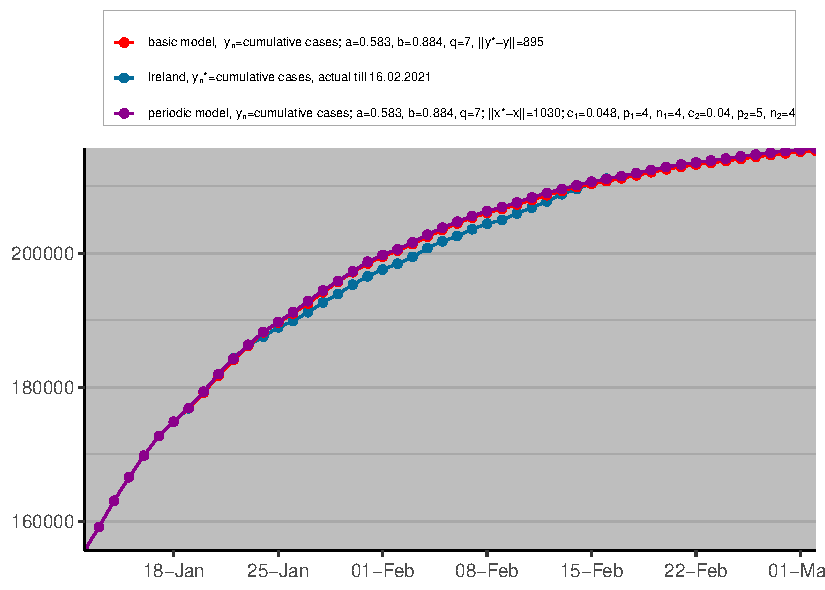
\includegraphics[width=\linewidth]{Ireland-periodicy.pdf} \label{fig:ireland-periodicy}
\endminipage
\caption{Periodic model, Ireland}
\end{figure}

\begin{figure}[H]
\minipage{0.48\textwidth}
  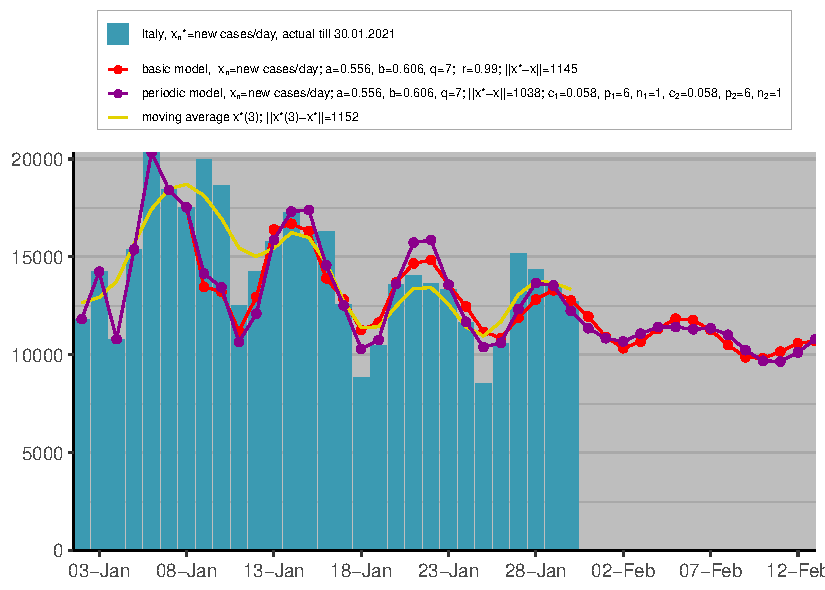
\includegraphics[width=\linewidth]{Italy-periodic.pdf} \label{fig:italy-periodic}
\endminipage\hfill
\minipage{0.48\textwidth}
  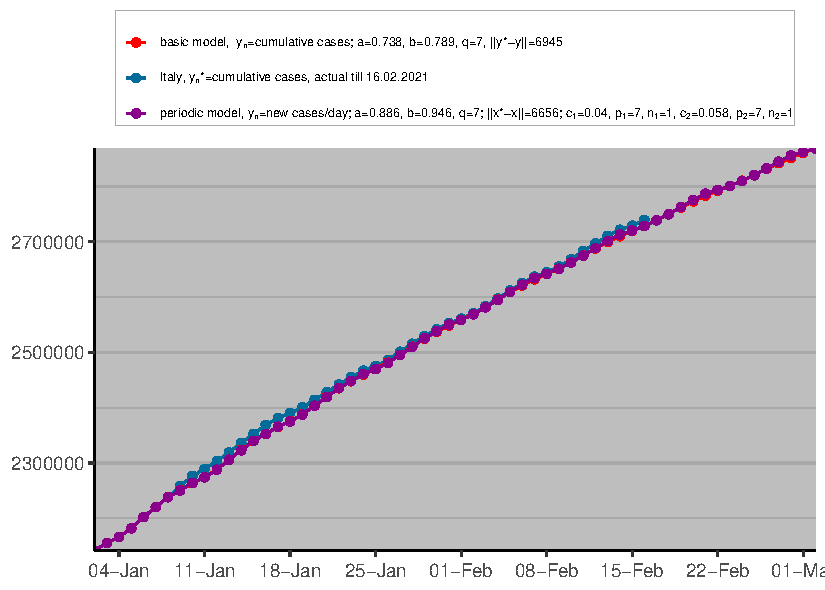
\includegraphics[width=\linewidth]{Italy-periodicy.pdf} \label{fig:italy-periodicy}
\endminipage
\caption{Periodic model, Italy}
\end{figure}

\begin{figure}[H]
\minipage{0.48\textwidth}
  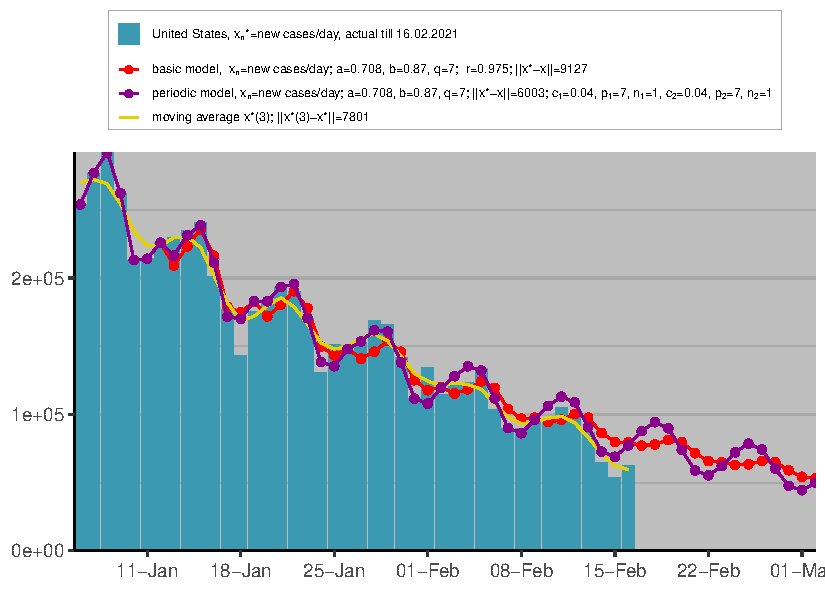
\includegraphics[width=\linewidth]{United States-periodic.pdf} \label{fig:usa-periodic}
\endminipage\hfill
\minipage{0.48\textwidth}
  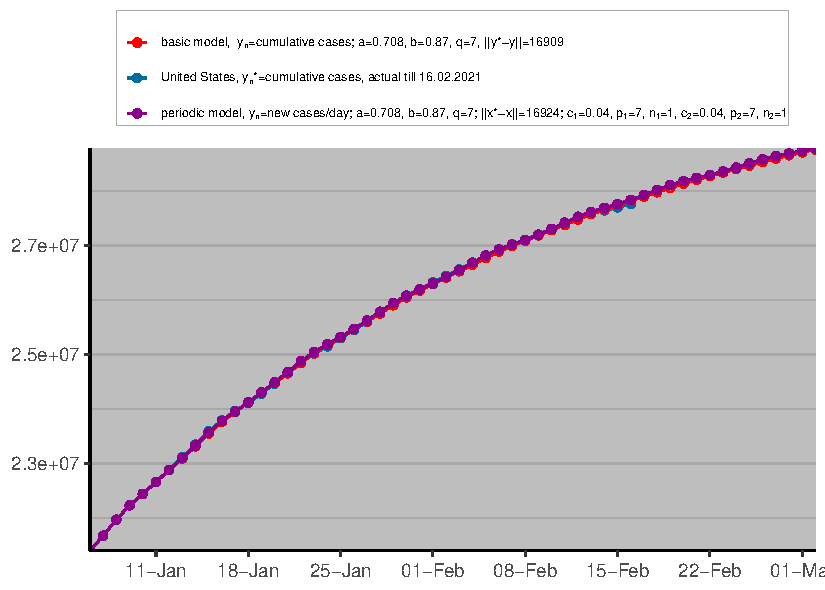
\includegraphics[width=\linewidth]{United States-periodicy.pdf} \label{fig:usa-periodicy}
\endminipage
\caption{Periodic model, United States}
\end{figure}

\subsection{Multi-phase model}

\subsubsection{Definitions and Theory}

\subsubsection{How to select the best model}

\subsubsection{Forecasting}

\subsubsection{Implementation in R}

\subsubsection{Plots}

The multi-phase model without periodicity can be sharp and unrealstic

\begin{figure}[H]
\minipage{0.48\textwidth}
  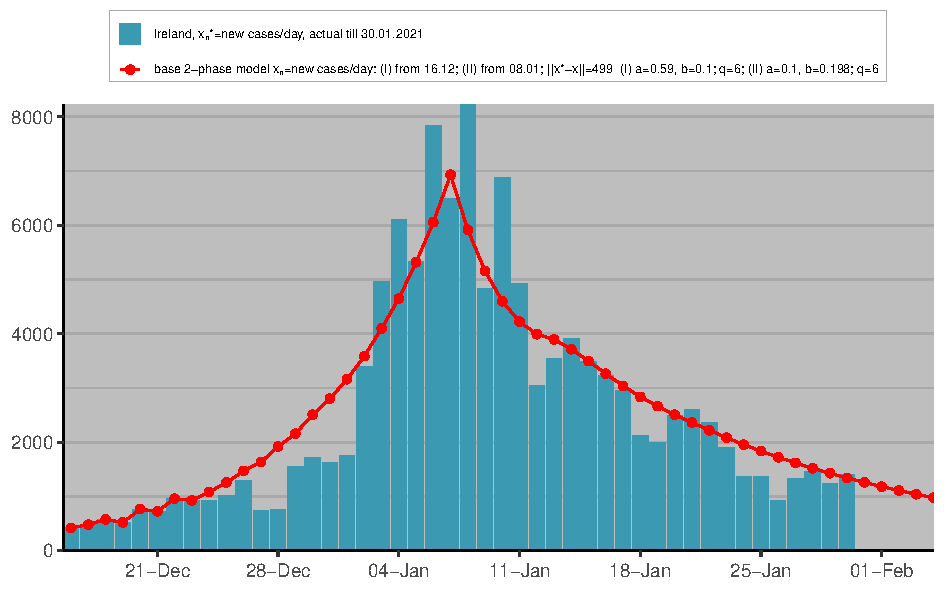
\includegraphics[width=\linewidth]{Ireland-xnmult.pdf} \label{fig:ireland-xnmult}
\endminipage\hfill
\minipage{0.48\textwidth}
  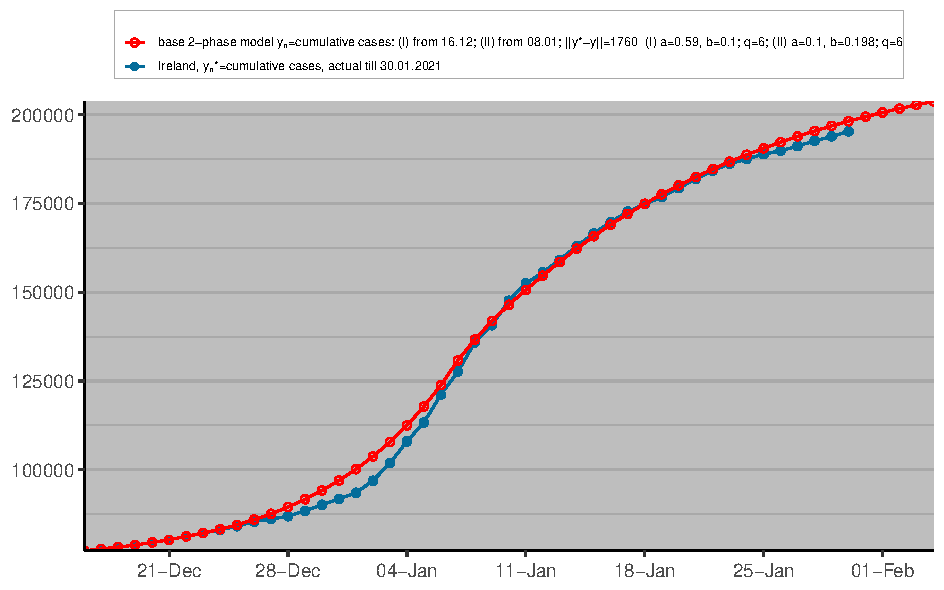
\includegraphics[width=\linewidth]{Ireland-ynmult.pdf} \label{fig:ireland-ynmult}
\endminipage
\caption{Multi-phase model, Ireland}
\end{figure}

\begin{figure}[H]
\minipage{0.48\textwidth}
  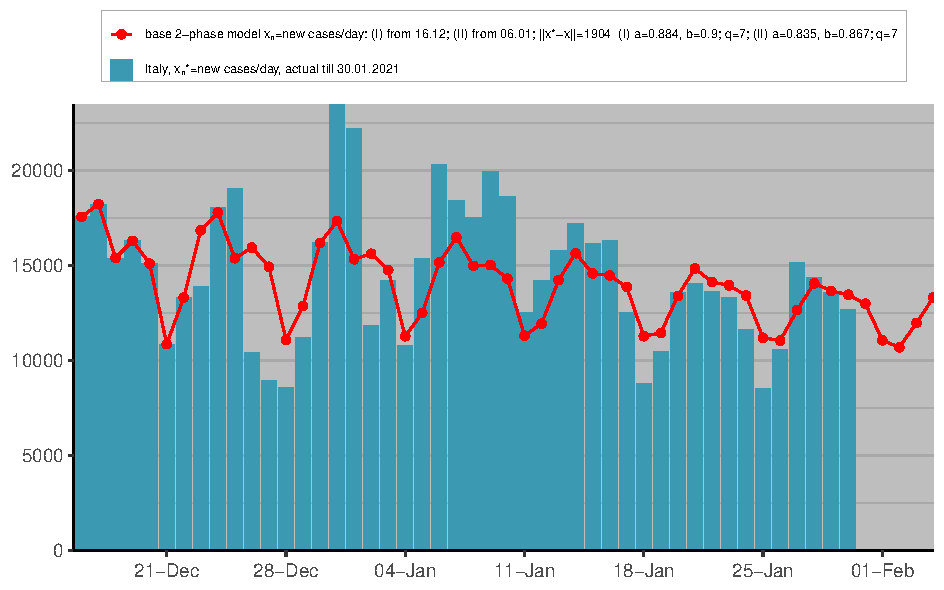
\includegraphics[width=\linewidth]{Italy-xnmult.pdf} \label{fig:italy-xnmult}
\endminipage\hfill
\minipage{0.48\textwidth}
  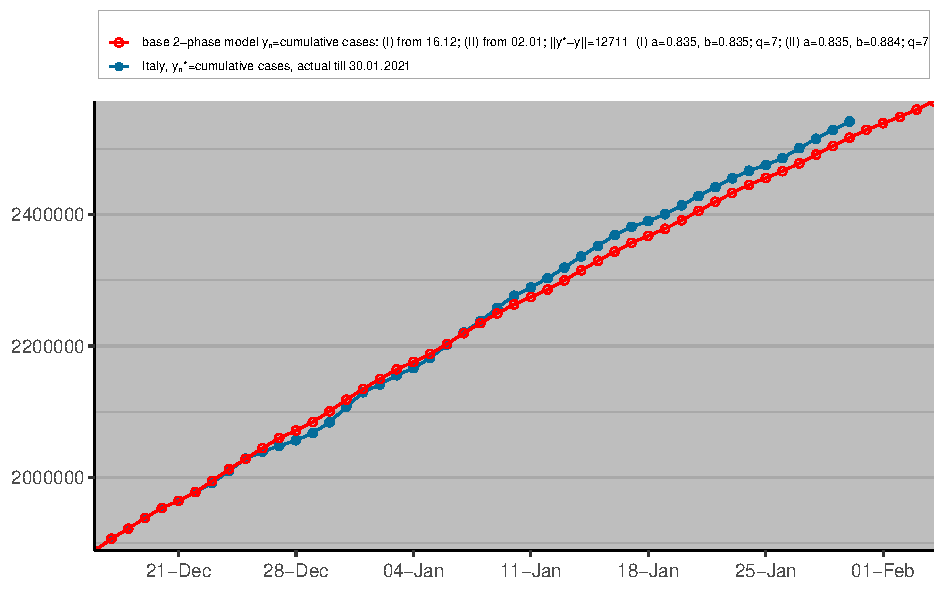
\includegraphics[width=\linewidth]{Italy-ynmult.pdf} \label{fig:italy-ynmult}
\endminipage
\caption{Multi-phase model, Italy}
\end{figure}

\begin{figure}[H]
\minipage{0.48\textwidth}
  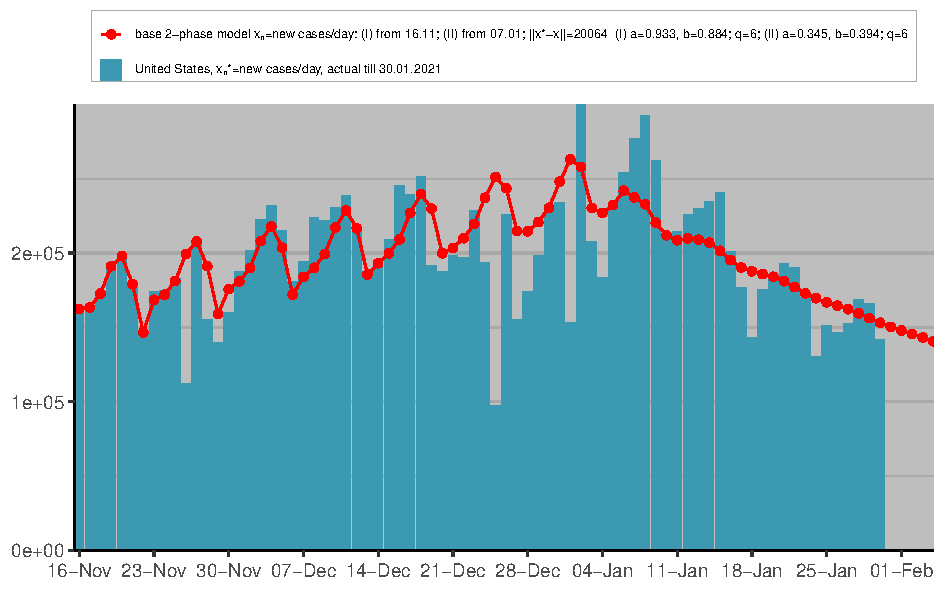
\includegraphics[width=\linewidth]{United States-xnmult.pdf} \label{fig:usa-xnmult}
\endminipage\hfill
\minipage{0.48\textwidth}
  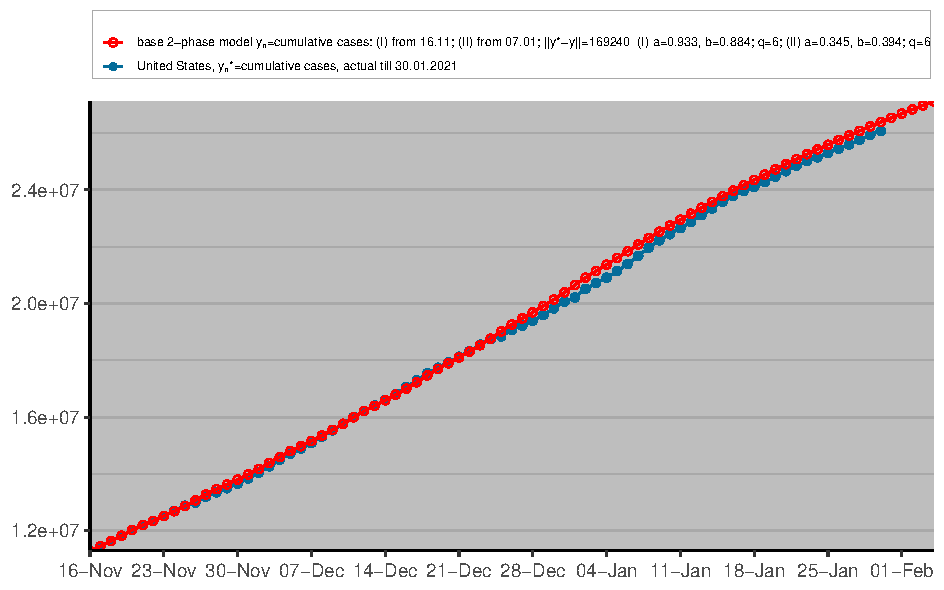
\includegraphics[width=\linewidth]{United States-ynmult.pdf} \label{fig:usa-ynmult}
\endminipage
\caption{Multi-phase model, United States}
\end{figure}


The periodic model often performs much better

\begin{figure}[H]
\minipage{0.48\textwidth}
  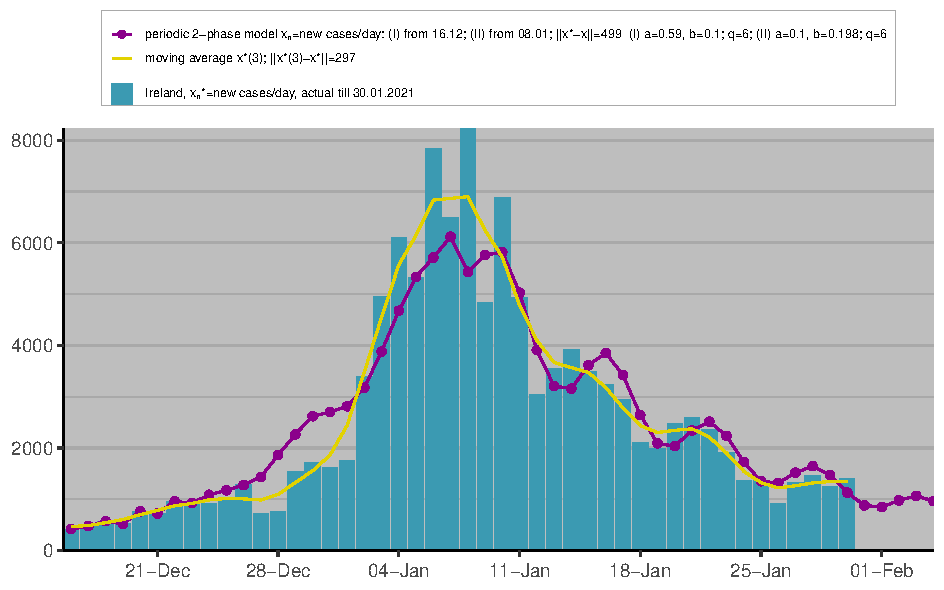
\includegraphics[width=\linewidth]{Ireland-perxnmult.pdf} \label{fig:ireland-perxnmult}
\endminipage\hfill
\minipage{0.48\textwidth}
  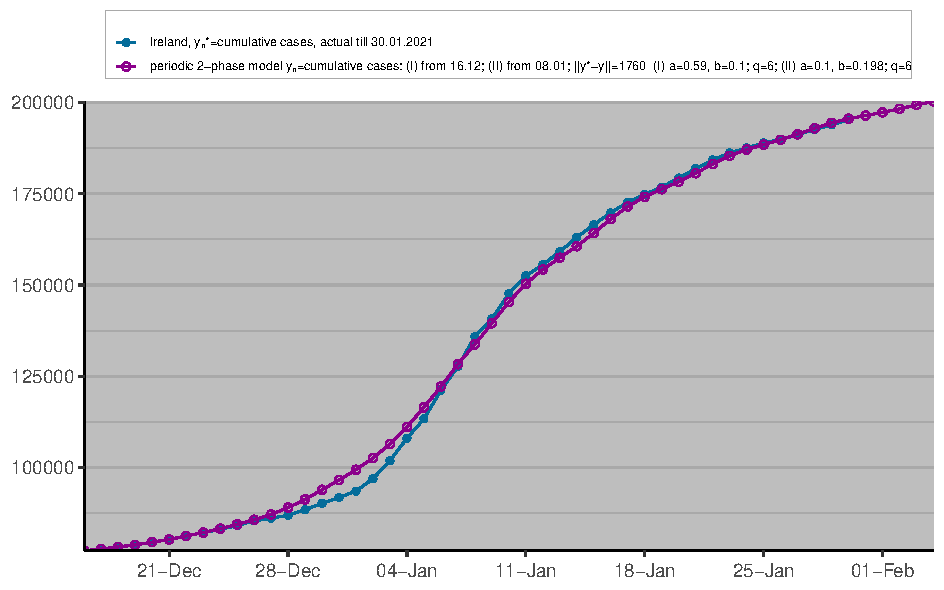
\includegraphics[width=\linewidth]{Ireland-perynmult.pdf} \label{fig:ireland-perynmult}
\endminipage
\caption{Multi-phase periodic model, Ireland}
\end{figure}

\begin{figure}[H]
\minipage{0.48\textwidth}
  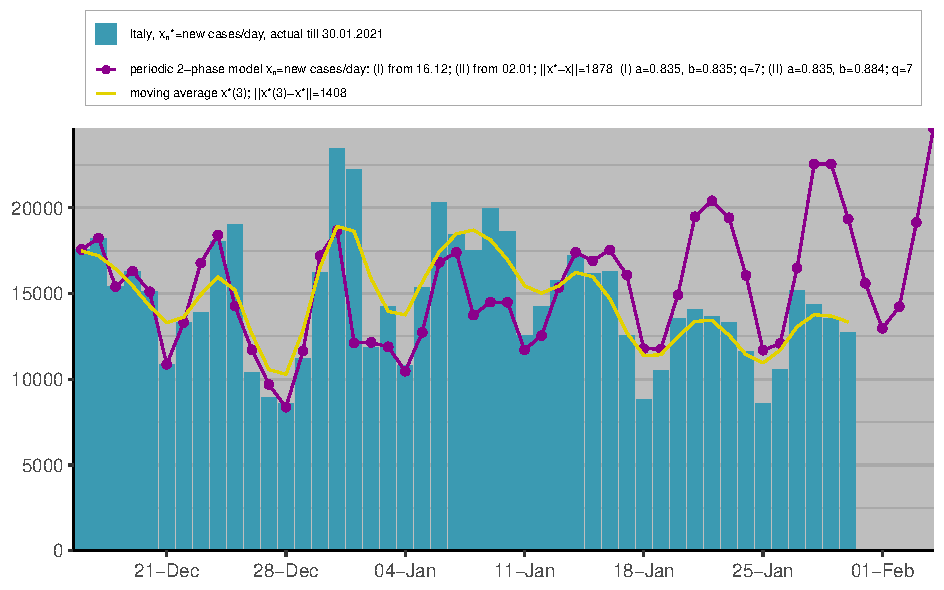
\includegraphics[width=\linewidth]{Italy-perxnmult.pdf} \label{fig:italy-perxnmult}
\endminipage\hfill
\minipage{0.48\textwidth}
  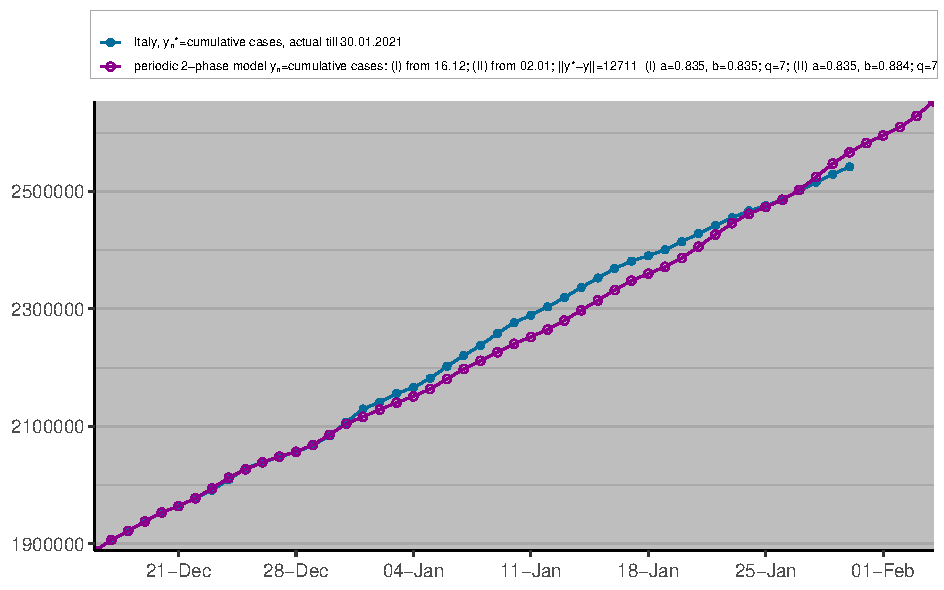
\includegraphics[width=\linewidth]{Italy-perynmult.pdf} \label{fig:italy-perynmult}
\endminipage
\caption{Multi-phase periodic model, Italy}
\end{figure}

\begin{figure}[H]
\minipage{0.48\textwidth}
  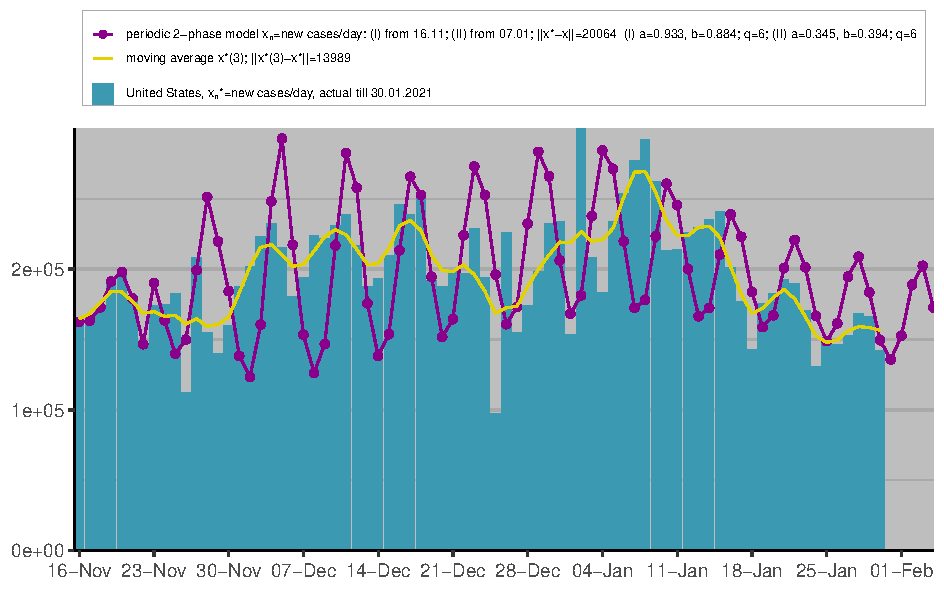
\includegraphics[width=\linewidth]{United States-perxnmult.pdf} \label{fig:usa-perxnmult}
\endminipage\hfill
\minipage{0.48\textwidth}
  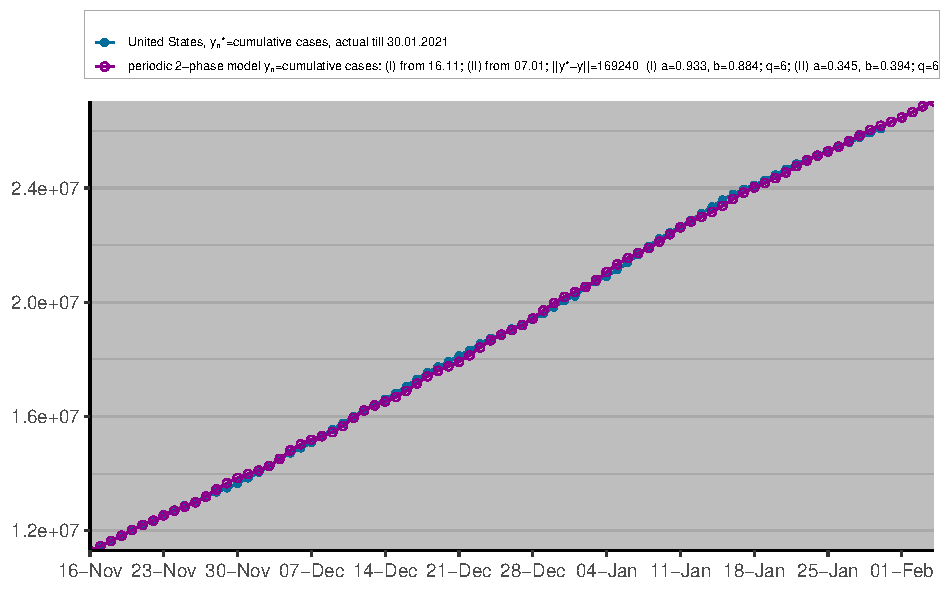
\includegraphics[width=\linewidth]{United States-perynmult.pdf} \label{fig:usa-perynmult}
\endminipage
\caption{Multi-phase periodic model, United States}
\end{figure}
